% Hard disk drive platter
% Author: Tomáš Michalek
%
% This diagram attempts to create HDD platter with the selectable track,
% sector and block highlighting.
%
%
% Improved thanks to the help of Qrrbrbirlbel <https://tex.stackexchange.com/users/16595/qrrbrbirlbel>
%
% https://tex.stackexchange.com/questions/696993/aligment-of-the-hightlight-in-the-tikz-figure/696999#696999

\documentclass[tikz, margin=10pt]{standalone}

\definecolor     {baseColor}{RGB}{ 18,  54,  69} % Basic lines and borders
\definecolor   {accentColor}{RGB}{  1, 103, 143} % Selection
\definecolor{highlightColor}{RGB}{221, 109,  16} % Crossover of two selections

\tikzset{
  ring segment/.style n args={4}{insert path={% helpful
       ({#1}:{#4}) arc[start angle={#1}, end angle={#2}, radius={#4}]
    -- ({#2}:{#3}) arc[start angle={#2}, end angle={#1}, radius={#3}] -- cycle}}}

\begin{document}
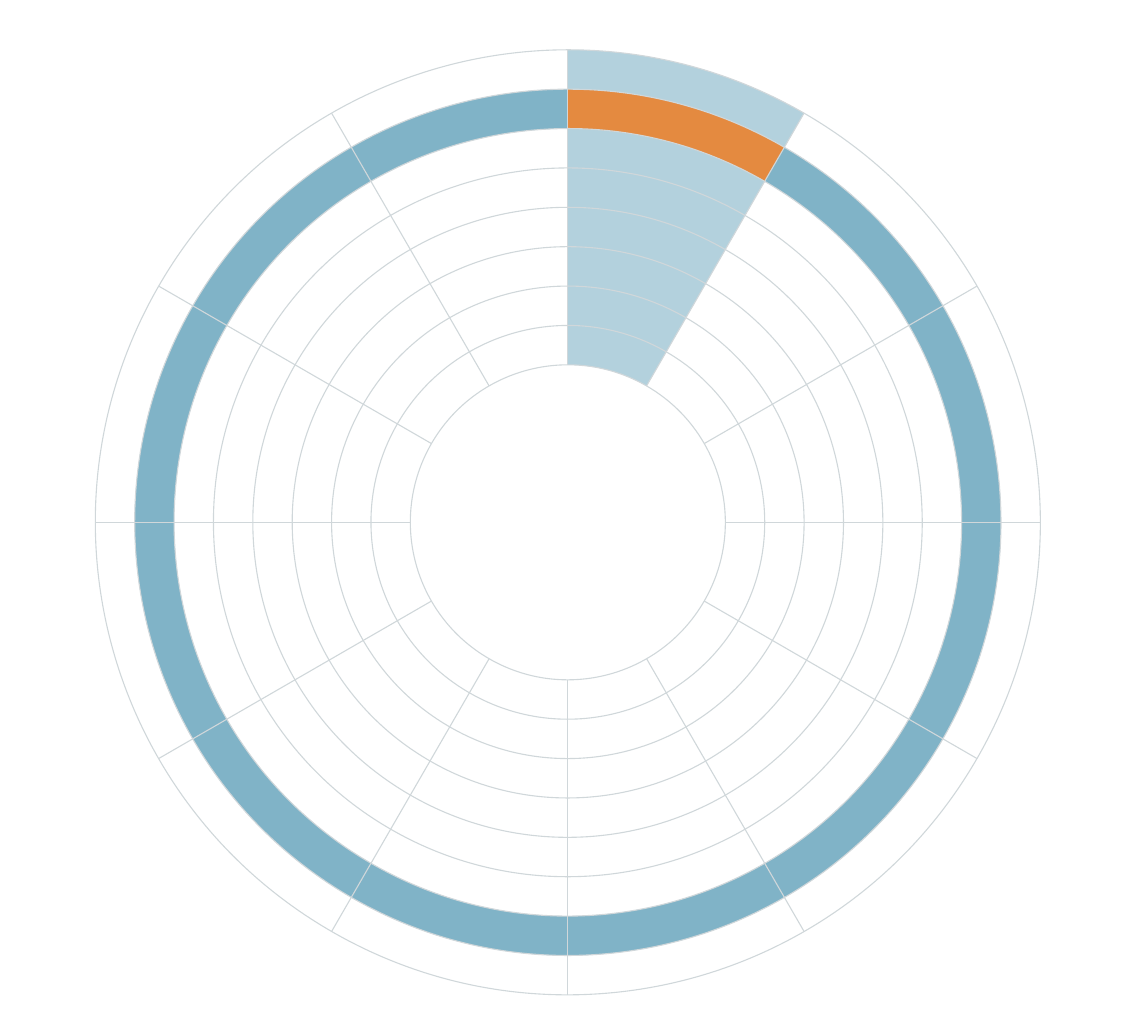
\begin{tikzpicture}[
  hdd border/.style    ={draw=     baseColor!20},
  hdd sel track/.style ={fill=   accentColor!50},
  hdd sel sector/.style={fill=   accentColor!30},
  hdd sel block/.style ={fill=highlightColor!80},
]
%%%%%%%%%%%%%%%%%%%%%%%%%%%%%%%%%%%%%%%%%%%%%%%%%%%%%%%%%%%%%%%%%%%%%%%%%%%%%%%%%%%%%%%%%
%
%   SETTINGS
%
%%%%%%%%%%%%%%%%%%%%%%%%%%%%%%%%%%%%%%%%%%%%%%%%%%%%%%%%%%%%%%%%%%%%%%%%%%%%%%%%%%%%%%%%%
\newcommand*\numTracks{8}
\newcommand*\numSectors{12}

\newcommand*\selectTrack{1}  % Track  to highlight, negative values disable the selection
\newcommand*\selectSector{1} % Sector to highlight, zero or lower values disable the selection

%%%%%%%%%%%%%%%%%%%%%%%%%%%%%%%%%%%%%%%%%%%%%%%%%%%%%%%%%%%%%%%%%%%%%%%%%%%%%%%%%%%%%%%%%
%
%   CALCULATIONS + HELPERS
%
%%%%%%%%%%%%%%%%%%%%%%%%%%%%%%%%%%%%%%%%%%%%%%%%%%%%%%%%%%%%%%%%%%%%%%%%%%%%%%%%%%%%%%%%%

\newcommand*\radiusBase{2}
\newcommand*\radiusStep{.5}

\ifnum\selectTrack>-1
    % Make the selected `track` behave more naturally
    \pgfmathtruncatemacro\selTrack{\numTracks-\selectTrack-1} 
\else
    \pgfmathtruncatemacro\selTrack{-1}
\fi

\ifnum\selectSector>0
    % Make the selected `sector` behave more naturally
    \pgfmathtruncatemacro\selSector{\numSectors-\selectSector+1} 
\else
    \pgfmathtruncatemacro\selSector{-1}
\fi

\pgfmathsetmacro\stepAngle{360/\numSectors}
\pgfmathsetmacro\radiusMax{\radiusBase+\numTracks*\radiusStep}
\pgfmathsetmacro\selectedAngleLower{\stepAngle*\selSector}
\pgfmathsetmacro\selectedAngleUpper{\selectedAngleLower+\stepAngle}
\pgfmathsetmacro\selectedRadiusLower{\radiusBase+\radiusStep*\selTrack}
\pgfmathsetmacro\selectedRadiusUpper{\selectedRadiusLower+\radiusStep}

%%%%%%%%%%%%%%%%%%%%%%%%%%%%%%%%%%%%%%%%%%%%%%%%%%%%%%%%%%%%%%%%%%%%%%%%%%%%%%%%%%%%%%%%%
%
%   DRAWING
%
%%%%%%%%%%%%%%%%%%%%%%%%%%%%%%%%%%%%%%%%%%%%%%%%%%%%%%%%%%%%%%%%%%%%%%%%%%%%%%%%%%%%%%%%%
\begin{scope}[rotate=2*\stepAngle] % Align starting point with `natural` selectors

    \ifnum\selTrack>-1
      \fill[hdd sel track, even odd rule]
        circle [radius=\selectedRadiusUpper] circle [radius=\selectedRadiusLower];
    \fi
    
    \ifnum\selSector>-1
      \fill[hdd sel sector, ring segment=\selectedAngleLower\selectedAngleUpper\radiusBase\radiusMax];
    \fi
    
    \ifnum\selTrack>-1 
        \ifnum\selSector>-1
            \fill[hdd sel block, ring segment=\selectedAngleLower\selectedAngleUpper\selectedRadiusLower\selectedRadiusUpper];
        \fi
    \fi
    
    %% borders on top
    \foreach \track in {0, ..., \numTracks}
      \draw[hdd border] (0,0) circle[radius=\radiusBase+\track*\radiusStep];
    
    \ifnum\selSector>-1
        \foreach[count=\i from 0] \sectors in {1, ..., \numSectors}
          \draw[hdd border] (\i*\stepAngle:\radiusBase) -- (\i*\stepAngle:\radiusMax);
    \fi
\end{scope}

\end{tikzpicture}
\end{document}
